\documentclass{article}
\usepackage[T1]{fontenc}
\usepackage{lmodern}
\usepackage{graphicx}
\usepackage{amsmath,amssymb}
\usepackage[a4paper,margin=2cm]{geometry}
\usepackage[absolute,overlay]{textpos}
\setlength{\TPHorizModule}{1mm}
\setlength{\TPVertModule}{1mm}
\usepackage[indonesian]{babel}
\usepackage{hyperref}
\setlength{\emergencystretch}{2em}
% unit: Halaman 76

\begin{document}

% === Halaman 76 (python/native) ===

3. Jika dua huruf tidak pada baris yang sama atau kolom yang sama, 

maka:

• huruf pertama diganti dengan huruf pada perpotongan baris huruf 

pertama dengan kolom huruf kedua. 

• huruf kedua diganti dengan huruf pada titik sudut keempat dari 

persegi panjang yang dibentuk dari tiga huruf yang digunakan sampai 

sejauh ini.

Bigram: hz

H

Z

Cipherteks: BW

B

W

76

% deskripsi: gambar native xref 274
\noindent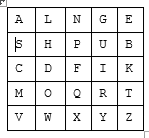
\includegraphics[width=0.85\textwidth]{../../images/python/page_076_img_01.png}

\end{document}
